\documentclass{standalone}

\usepackage{circuitikz}

\begin{document}

% INT_AY20_MP2_L21_Fig01-Rotation_plane.png

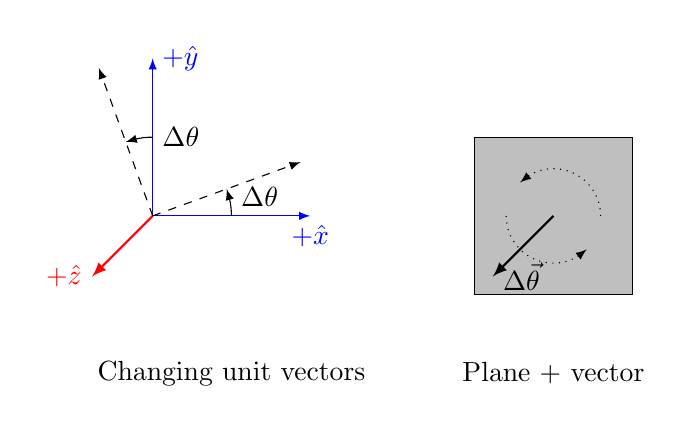
\begin{tikzpicture}[> = latex]

% Definitions

\def\L{2}		% Vector lengths
\def\Q{20}		% Amount of rotation

\matrix[column sep = 1 cm]{
	
	% Rotation axis
	
	\draw [->, thick, red] (0, 0, 0) -- (0, 0, \L) node [left] {$+{\hat z}$};
	
	% Original vectors
	
	\draw [->, blue] (0, 0, 0) -- (\L, 0, 0) node [below] {$+{\hat x}$};
	\draw [->, blue] (0, 0, 0) -- (0, \L, 0) node [right] {$+{\hat y}$};
	
	% Rotated vectors
	
	\draw [->, dashed] (0, 0, 0) -- ({\L * cos(\Q)}, {\L * sin(\Q)}, 0);
	\draw [->, dashed] (0, 0, 0) -- ({-\L * sin(\Q)}, {\L * cos(\Q)}, 0);
	
	% Angle indicators
	
	\draw [->] (0.5 * \L, 0, 0) node [above right] {$\Delta \theta$} arc (0 : \Q : {0.5 * \L});
	\draw [->] (0, 0.5 * \L, 0) node [right] {$\Delta \theta$} arc (90 : 90 + \Q : {0.5 * \L});
	
	% Label
	
	\node at (0.5 * \L, -\L) {Changing unit vectors};
	
&
	
	% Rotation plane
	
	\draw [fill = gray!50] (-0.5 * \L, -0.5 * \L, 0) -- (0.5 * \L, -0.5 * \L, 0) -- (0.5 * \L, 0.5 * \L, 0) -- (-0.5 * \L, 0.5 * \L) -- cycle;

	% Rotation directions
	
	\draw [->, dotted] (-0.3 * \L, 0, 0) arc (180 : 315 : {0.3 * \L});
	\draw [->, dotted] (0.3 * \L, 0, 0) arc (0 : 135 : {0.3 * \L});

	% Angular displacement vector
	
	\draw [->, thick] (0, 0, 0) -- (0, 0, \L) node [right] {$\Delta {\vec \theta}$};
	
	% Label
	
	\node at (0, -\L) {Plane + vector};

\\	
};

\end{tikzpicture}

\end{document}